\documentclass[11pt, oneside]{article}
\usepackage{geometry}
\geometry{
 a4paper,
 total={175mm,243mm},
 left=17mm,
 top=20mm,
 }

\usepackage{graphicx}	
\usepackage{amsmath}
\usepackage{amsfonts}
\usepackage{amssymb}
\usepackage{mathrsfs}
\usepackage{dsfont}
\usepackage{enumitem}

\usepackage{physics}
\usepackage{siunitx}
\usepackage{slashed}

\usepackage{tensor}

\usepackage{tikz}
\usetikzlibrary{shapes.geometric}

\newcommand{\G}{\Gamma}

\renewcommand\thesection{Exercise \arabic{section}:}

\title{ENS M1 General Relativity - Midterm Problems Solutions}
\author{Matteo Vilucchio}					

\begin{document}
\maketitle

\section{Divergence and Laplacian}
\begin{enumerate}
\item From the definition:
\begin{align*}
	\div{\va{V}} = \nabla_\mu V^\mu &= \partial_\mu V^\mu + \G_{\mu\gamma}^\mu V^\gamma = \partial_\mu V^\mu + \frac{1}{2} g^{\mu\nu}\qty( \partial_\mu g_{\nu\gamma} + \partial_\gamma g_{\nu\mu} - \partial_\nu g_{\mu\gamma})V^\gamma \\
	&= \partial_\mu V^\mu + \frac{1}{2} g^{\mu\nu}\partial_\gamma g_{\mu\nu} V^\gamma
\end{align*}

\item The metric transforms as a $(0,2)$ tensor and its inverse transforms as a $(2,0)$ tensor. To deduce how $c^{\mu\nu}$ transforms one should verify how $g$ transforms. Under a generic change of coordinates $g^{\mu\nu}$ becomes:
\[
	g^{\mu'\nu'} = \pdv{x^{\mu'}}{x^{\mu}} \pdv{x^{\nu'}}{x^{\nu}} g^{\mu\nu}
\]
and then by taking the determinant of both the RHS and the LHS one obtains:
\[
	g' = g \: \abs{\pdv{x^{\mu'}}{x^{\mu}}}^2
\]
where the absolute values is the determinant of the jacobian matrix. Since the change in coordinates can be arbitrary one can conclude that the cofactor matrix do not transform as a tensor.

\item The determinant of a $4\times4$ matrix can be written as:
\[
	g = \epsilon^{\mu\nu\gamma\rho} g_{0\mu} g_{1\nu} g_{2\gamma} g_{3\sigma}
\]
and then by differentiating one gets the actual definition of a minor:
\[
	\pdv{g}{g_{\rho\sigma}} = \epsilon^{\sigma\nu\gamma\delta} g_{\tau \nu}g_{\eta \gamma} g_{\pi\delta} = c^{\rho\sigma} \quad \tau, \eta, \pi \neq \rho
\]
The indices $\tau$, $\eta$ and $\pi$ are not summed over.

\item By applying the chain rule to the following:
\[
	\partial_\gamma g = \pdv{g}{g_{\mu\nu}} \partial_\gamma g_{\mu\nu} = g\: g^{\mu\nu}\:\partial_\gamma g_{\mu\nu}
\]
then by looking at the previous equation one can see that the only solution is the natural logarithm. So one obtains that:
\[
	g^{\mu\nu} \partial_\gamma g_{\mu\nu} = \partial_{\gamma}\qty( \ln \abs{g})
\]

\item The important notion to realise to make this point is that:
\[
	\frac{1}{\sqrt{\abs{g}}} \partial_\gamma \qty(\sqrt{\abs{g}}V^\gamma) = \frac{1}{\sqrt{\abs{g}}} \partial_\gamma \qty(\sqrt{\abs{g}}) V^\gamma + \frac{\sqrt{\abs{g}}}{\sqrt{\abs{g}}} \partial_\gamma V^\gamma = \frac{1}{2} \frac{1}{\abs{g}} \partial_\gamma g \: V^\gamma + \partial_\gamma V^\gamma = \frac{1}{2} \partial_{\gamma}\qty( \ln \abs{g}) + \partial_\gamma V^\gamma
\]
where the last part is exactly what has already been obtained in point 1. In the end one can read that:
\[
	\div \va{V}=\frac{1}{\sqrt{|g|}} \partial_{\gamma}\left(\sqrt{|g|} V^{\gamma}\right)
\]

\item This exercice is about writing the laplacian in a handy way. One can do it in two different ways:
\[
	\laplacian f = \div \grad f = \nabla_\mu \nabla^\mu \qty(f) = \nabla^\mu \nabla_\mu \qty(f)
\]
to apply the previous formula one has to choose the first proposition since the formula we have derived only applies to vectors. By recalling that the covariant derivative of a scalar function is just the partial derivative one can obtain:
\[
	\laplacian f = \frac{1}{\sqrt{|g|}} \partial_{\gamma}\qty(\sqrt{|g|} \partial^\gamma f) = \frac{1}{\sqrt{|g|}} \partial_{\gamma}\qty(\sqrt{|g|} g^{\gamma\mu}\partial_\mu f)
\]

\item In spherical coordinates the matrix associated with the metric is:
\[
	\qty[g_{\mu\nu}] = 
	\begin{bmatrix} 
	1 & 0 & 0 \\
	0 & r^2 & 0 \\
	0 & 0 & r^2 \sin^2 \theta
	\end{bmatrix}
\]
where a choice of basis has been made. The choice of this basis is the standard one w.r.t. the cartesian basis. From this the determinant reads as:
\[
	g = r^4 \sin^2 \theta
\]
This determinant is non zero for $r>0$ and for $\theta \in \:]0, \pi[$. In this region one can find the inverse matrix which is:
\[
	\qty[g^{\mu\nu}] = 
	\begin{bmatrix} 
	1 & 0 & 0 \\
	0 & \frac{1}{r^2} & 0 \\
	0 & 0 & \frac{1}{r^2 \sin^2 \theta}
	\end{bmatrix}
\]
then by applying the formulas obtained in point 6 one can directly have the expressions for the laplacian of a scalar function in spherical coordinates.
\begin{align*}
	\laplacian f &= \frac{1}{r^2\sin\theta} \partial_\gamma\qty( r^2\sin\theta  g^{\gamma\mu}\partial_\mu f) = \\
	&= \frac{1}{r^2\sin\theta} \partial_r \qty(r^2\sin\theta g^{rr} \partial_r f) + \frac{1}{r^2\sin\theta} \partial_r \qty(r^2\sin\theta g^{\theta\theta} \partial_\theta f) + \frac{1}{r^2\sin\theta} \partial_\phi \qty(r^2\sin\theta g^{\phi\phi} \partial_\phi f) = \\
	&= \frac{1}{r^2} \partial_r \qty( r^2 \:\partial_r f ) + \frac{1}{r^2 \sin\theta} \partial_\theta \qty( \sin\theta \:\partial_\theta f ) + \frac{1}{r^2\sin^2\theta}\partial_\phi^2 f
\end{align*}

\item In cylindrical coordinates one has that the metric and its inverse are:
\[
	\qty[g_{\mu\nu}] = 
	\begin{bmatrix} 
	1 & 0 & 0 \\
	0 & r^2 & 0 \\
	0 & 0 & 1
	\end{bmatrix}
	\qquad 
	\qty[g^{\mu\nu}] = 
	\begin{bmatrix} 
	1 & 0 & 0 \\
	0 & \frac{1}{r^2} & 0 \\
	0 & 0 & 1
	\end{bmatrix}
	\qquad
	g = r^2
\]
and the range of validity for the existence of the inverse matrix is $r>0$. Then the laplacian in cylindrical coordinates becomes:
\[
	\laplacian f = \frac{1}{r} \partial_r \qty( r \partial_r f) + \frac{1}{r^2} \partial_\phi^2 f + \partial_z^2 f
\] 

\end{enumerate}


\section{Rotating coordinate frame}
\begin{enumerate}
\item Intuitively one can say that the change in frame will "mix up" the angular and temporal coordinates. By looking specifically at the change of variables one has that:
\[
	\begin{cases}
		z = z' \\
		r = r' \\
		\phi = \phi' - \Omega t \\
		t = t' \\ 
	\end{cases}
	\iff
	\begin{cases}
		\dd{z} = \dd{z'} \\
		\dd{r} = \dd{r'} \\
		\dd{\phi} = \dd{\phi'} - \Omega \dd{t} \\
		\dd{t} = \dd{t'}
	\end{cases}
\]
then by substituting the differentials inside the line element one obtains the expression for the invariant in the other frame of reference:
\[
	d s^2 = \qty(r^2\Omega^2 - c^2) \dd{t}^2 + 2\Omega r^2 \dd{t} \dd{\phi}+ r^2 \dd{\phi}^2 + \dd{r}^2 + \dd{z}^2
\]
and in matrix form the metric becomes:
\[
	\qty[g_{\mu\nu}] = 
	\begin{bmatrix}
		r^2\Omega^2 - c^2 & 0 &\Omega r^2 & 0 \\
		0 & 1 & 0 & 0 \\
		\Omega r^2 & 0 & r^2 & 0 \\
		0 & 0 & 0 & 1 \\
	\end{bmatrix}
\]

\item The inverse of this matrix becomes:
\[
	\qty[g^{\mu\nu}] = 
	\begin{bmatrix}
		-\frac{1}{c^{2}} & 0 & \frac{\Omega}{c^{2}} & 0 \\
		0 & 1 & 0 & 0 \\
		\frac{\Omega}{c^{2}} & 0 & \frac{1}{r^{2}} -\frac{\Omega^{2}}{c^{2}} & 0 \\
		0 & 0 & 0 & 1
	\end{bmatrix}
\]

\item The line element in the primed frame in cartesian coordinates is:
\[
	ds'^2 = -c^2\dd{t}'^2 + \dd{x}'^2 + \dd{y} '^2 + \dd{z}'^2
\]
Next one should evaluate how the differentials change under the change of coordinates. The only one that change are the following:
\begin{align*}
	\dd{x'} &= \cos\Omega t \dd{x} + \sin\Omega t \dd{y} + \Omega \qty(\cos\Omega t \:y - \sin \Omega t\:x) \dd{t} \\
	\dd{y'} &= -\sin\Omega t \dd{x} + \sin\Omega t \dd{y} - \Omega \qty(\cos\Omega t \:x + \sin \Omega t\:y) \dd{t}
\end{align*}
and their squares are:
\begin{align*}
	\dd{x'}^2 &= \cos^2\Omega t  \dd{x}^2 + \sin^2 \Omega t \dd{y}^2 + \Omega^2 \qty(\cos\Omega t \:y - \sin \Omega t\:x)^2 \dd{t}^2 + \\
	& \quad + 2\Omega\qty(\cos\Omega t \:y - \sin \Omega t\:x) \cos\Omega t \dd{x} \dd{t} \\
	& \quad + 2\Omega\qty(\cos\Omega t \:y - \sin \Omega t\:x) \sin\Omega t \dd{y} \dd{t} \\
	& \quad + 2 \cos\Omega t \sin\Omega t \dd{x} \dd{y} \\
	\dd{y'}^2 &= \sin^2 \Omega t  \dd{x}^2 + \cos^2\Omega t \dd{y}^2 + \Omega^2 \qty(\cos\Omega t \:x + \sin \Omega t\:y)^2 \dd{t}^2 +\\
	& \quad + 2\Omega\qty(\cos\Omega t \:x + \sin \Omega t\:y)  \sin\Omega t \dd{x} \dd{t}  \\
	& \quad - 2\Omega\qty(\cos\Omega t \:x + \sin \Omega t\:y) \cos\Omega t \dd{y} \dd{t}\\
	& \quad - 2 \cos\Omega t \sin\Omega t \dd{x} \dd{y} \\
\end{align*}
Then by inserting this expression in the line element:
\[
	d s^2 = \qty(-c^2 + \Omega^2(x^2 + y^2)) \dd{t}^2 + \dd{x}^2 + \dd{y}^2 + 2 \Omega y \dd{x} \dd{t} - 2 \Omega x  \dd{y} \dd{t} 
\]
and then the metric becomes:
\[
	\qty[g_{\mu\nu}] = 
	\begin{bmatrix}
		\Omega^2\qty(x^2 + y^2) - c^2 & \Omega y & -\Omega x & 0 \\
		\Omega y & 1 & 0 & 0 \\
		-\Omega x & 0 & 1 & 0 \\
		0 & 0 & 0 & 1 \\
	\end{bmatrix}
\]
where the order of the coordinates is: time, $x$ , $y$ and $z$.

\item By assuming that the difference between the above written metric and the minkowskian metric is small this difference can be written as:
\[
	\qty[h_{\mu\nu}] = 
	\begin{bmatrix}
		\Omega^2\qty(x^2 + y^2)& \Omega y & -\Omega x & 0 \\
		\Omega y & 0 & 0 & 0 \\
		-\Omega x & 0 & 0 & 0 \\
		0 & 0 & 0 & 0 \\
	\end{bmatrix}
\]
Then, at first order, the connection coefficients can be written in a simpler way:
\[
	\G_{\mu\lambda}^\nu = \frac{1}{2} \eta^{\nu\gamma}\qty(\partial_\mu h_{\gamma\lambda} + \partial_{\lambda}h_{\gamma\mu} - \partial_\gamma h_{\lambda\mu} )
\]
From the previous expression we know that $h_{\mu\nu}$ depends only on the coordinates $x$ and $y$. Then the only non zero coefficients at first order will be:
\begin{align*}
	\G^{x}_{00} &= \frac{1}{2} \eta^{x\lambda} \qty(2\partial_0 h_{0\lambda} - \partial_\lambda h_{00}) = -\frac{1}{2} \eta^{x\lambda} \partial_\lambda h_{00} = -\frac{1}{2} \eta^{xx} 2\Omega^2 x -\frac{1}{2} \eta^{xy} 2\Omega^2 y = \\
	&= -\Omega^2 x \\
	\G^{y}_{00} &= \frac{1}{2} \eta^{y\lambda} \qty(2\partial_0 h_{0\lambda} - \partial_\lambda h_{00}) = -\frac{1}{2} \eta^{y\lambda} \partial_\lambda h_{00} = -\frac{1}{2} \eta^{yx} 2\Omega^2 x -\frac{1}{2} \eta^{yy} 2\Omega^2 y =  \\
	&= -\Omega^2 y \\
	\G^{x}_{0y} &= \frac{1}{2} \qty(\partial_0 h_{yx} + \partial_y h _{0x} - \partial_x h_{0y}) = \Omega \\
	\G^{y}_{0x} &= \frac{1}{2} \qty(\partial_0 h_{yx} + \partial_x h _{0y} - \partial_y h_{0x}) = -\Omega 
\end{align*}

Where one can use that, up to first order, the inverse of the metric is $\eta^{\mu\nu} - h^{\mu\nu}$.

\item In this case to find the equations of motions the geodesic equations read:
\[
	\begin{cases}
		\ddot{x} = -\G^{x}_{\alpha\beta} \:\dot{x^\alpha} \dot{x^\beta} = \Omega^2 x - \Omega \dot{y} \\
		\ddot{y} = -\G^{y}_{\alpha\beta} \:\dot{x^\alpha} \dot{x^\beta} = \Omega^2 y + \Omega \dot{x} \\
	\end{cases}
\]
This equations are similar to the equation that one would obtain for an harmonic oscillator with a Coriolis force, a physical example is a linearised Focalult's pendulum.
\end{enumerate}

\section{Frame dragging by a moving rod}
\begin{enumerate}
\item The equation for $\Phi$ is the same as the equation that regulates the behaviour of an electric potential in the presence of an infinite charged cylinder. One useful notation used below is rewriting the equation as:
\[
	\laplacian \Phi = 4\pi \qty(\frac{G_N}{c^2}) \rho(r) \equiv \alpha \Theta(R-r)
\]
with the use of the Heaviside Theta distribution. Then in general the potential we are looking for is:
\[
	\Phi(r) = 
	\begin{cases}
		\frac{\alpha}{4} r^2 + V_0 & r \leq R \\
		\frac{\alpha}{4} R^2 +\frac{\alpha}{2} R^2 \ln\qty(\frac{r}{R}) + V_0& r \geq R
	\end{cases}
\]
and by choosing the constant $V_0$ as $-\alpha/4 R^2$ both the boundary conditions are satisfied. Another way to obtain the same result is to directly solve the equation for the $r$ coordinate. In the other directions, by imposing the right boundary conditions, one can see that it should not depend on them. The laplacian equation becomes:
\[
	\frac{1}{r} \qty( \pdv{r} \qty(r \pdv{\Phi}{r})) = \alpha \Theta (R- r)
\]
So solving the equation inside the cylinder:
\[
	r \pdv{\Phi}{r} = \alpha \frac{r^2}{2} + C
\]
by imposing the boundary condition on the derivative one gets that $C=0$. And then one has that integrating once again and imposing the boundary condition:
\[
	\Phi_{r<R} = \frac{\alpha}{4} \qty(r^2 - R^2) = \pi \qty(\frac{G_N}{c^2}) \qty(r^2 - R^2)
\]
Outside the cylinder one has to solve Laplace equation, and the solution that satisfy the boundary condition (that is also continuous at the intersection point) is:
\[
	\Phi_{r>R} = \frac{\alpha}{2}R^2 \log \qty(\frac{r}{R})
\]

\item To solve for the $h$ one should invert the relation for the trace inverse as follows:
\[
	h_{\mu\nu} = \overline{h}_{\mu\nu} - \frac{1}{2} \eta_{\mu\nu} \overline{h} = -4 \Phi(r) \delta^{0}_{~\mu}\delta^{0}_{~\nu} + 2 \eta_{\mu\nu} \Phi(r) = - 2 \Phi(r) \delta_{\mu\nu}
\]

\item The change of variables it is going to be introduced is the following:
\[
	\begin{cases}
		r^{\prime}=\left(1+r \pdv{\Phi}{r}\right)(1-\Phi) r =  r (\frac{1}{2}-\frac{\alpha}{4})\left(2-\alpha \log \qty(\frac{r}{R})\right)\\
		\phi^{\prime}=\left(1-r \pdv{\Phi}{r} \right) \phi = \qty(1 - \frac{\alpha}{2})\phi
	\end{cases}
\]
With the change of variable given the differentials become:
\begin{align*}
	\dd{r'}^2 + r'^2 \dd{\phi'}^2 = \frac{1}{64}(-2+\alpha)^{2}\left(r^{2}(2+\alpha)^{2} \dd{\phi}^{2}\left(2+\alpha \log \qty(\frac{r}{R})\right)^{2}+4 \dd{r}^{2}\left(2+\alpha+\alpha \log \qty(\frac{r}{R})\right)^{2}\right)
\end{align*}
which can be linearised in a first order theory to obtain:
\[
	\dd{r'}^2 + r'^2 \dd{\phi'}^2 \simeq \left(\dd{r}^{2}+r^{2} \dd{\phi}^{2}\right)\left(1-\alpha \log \qty(\frac{r}{R})\right)
\]
One important point is that the new angular variable $\phi'$ has a range smaller than $[0, 2\pi]$. From the previous change of variables one can see that the epsilon is $ 4\pi G_N \mu / c^2$.

\item 
\begin{enumerate}[label=(\alph*)]
	\item The transformation matrix is:
	\[
		[\Lambda^{\mu}_{~\nu}]=\left(\begin{array}{cccc}
			\gamma & 0 & 0 & \beta \gamma \\
			0 & 1 & 0 & 0 \\
			0 & 0 & 1 & 0 \\
			\beta \gamma & 0 & 0 & \gamma
		\end{array}\right)
	\]
	\item To show that it is the right transformation one can consider the following:
	\[
		\Lambda \begin{pmatrix}
			ct \\
			0 \\
			0 \\
			0 
		\end{pmatrix} =
		\begin{pmatrix}
			\frac{c t}{\sqrt{1-\frac{v^{2}}{c^{2}}}} \\
			 0 \\
			 0 \\
			 \frac{tv}{\sqrt{1-\frac{v^{2}}{c^{2}}}}
		\end{pmatrix}
	\]
	which represent a point that travels in the positive $x^3$ direction as time passes.
	
	\item Well, to find the transformation proprieties of a covariant $(0,2)$-tensor one can consider the scalar invariant $t_{\alpha\beta}x^{\alpha}x^{\beta}$. Then:
	\[
		t_{\alpha\beta}x^{\alpha}x^{\beta} = t_{\alpha'\beta'}x^{\alpha'}x^{\beta'} = t_{\alpha'\beta'} \Lambda^{\alpha'}_{~\alpha} x^{\alpha}  \Lambda^{\beta'}_{~\beta} x^{\beta}
	\]
	and so by comparison between the first and the last term:
	\[
		t_{\alpha\beta} = t_{\alpha'\beta'} \Lambda^{\alpha'}_{~\alpha}\Lambda^{\beta'}_{~\beta} \implies t_{\alpha'\beta'} = \Lambda^{~\alpha}_{\alpha'} \Lambda^{~\beta}_{\beta'} t_{\alpha\beta}
	\]
	where the notation utilised is that $\Lambda_{\beta'}^{~\beta}$ is the inverse metric defined as:
	\[
		[\Lambda_{\mu}^{~\nu}] = \begin{pmatrix}
			\gamma & 0 & 0 & -\beta \gamma \\
			0 & 1 & 0 & 0 \\
			0 & 0 & 1 & 0 \\
			-\beta \gamma & 0 & 0 & \gamma
		\end{pmatrix}
	\]
	
	\item In this way one can find the transformed perturbation to the metric.
	\[
		[h_{\alpha'\beta'}] = \frac{\alpha}{2} \log \qty(\frac{r}{R}) \begin{pmatrix}
			\frac{c^{2}+v^{2}}{c^{2}-v^{2}} & 0 & 0 & -\frac{2 c v}{c^{2}-v^{2}} \\
			0 & 1 & 0 & 0 \\
			0 & 0 & 1 & 0 \\
			-\frac{2 c v}{c^{2}-v^{2}} & 0 & 0 & \frac{c^{2}+v^{2}}{c^{2}-v^{2}}
		\end{pmatrix}
	\]
	
\end{enumerate}

\item With a Taylor expansion of $h_{\alpha'\beta'}$ in the terms of $v/c$ one finds that:
\[
	h_{\alpha'\beta'} = \frac{\alpha}{2} \log \qty(\frac{r}{R}) \begin{pmatrix}
		1 & 0 & 0 & -2\beta \\
		0 & 1 & 0 & 0 \\
		0 & 0 & 1 & 0 \\
		-2\beta & 0 & 0 & 1
	\end{pmatrix}
	+ \order{\beta^2}
\] 

\begin{figure}[htbp]
   \centering
   \includegraphics[scale=0.65]{zeta.png} % requires the graphicx package
   \caption{Displacement in the $z$ direction. The simulation has been carried out with the following paramethers: $R=1\si{\meter}$, $v=\SI{1e5}{\meter\per\second}$, $\rho_0 = \SI{1e20}{\kilo\gram\per\meter\cubed}$, $x_0 = 11\si{\meter}$ and $\dot{x}_0 = \SI{-1e5}{\meter\per\second}$.}
   \label{fig:zeta}
\end{figure}

\item 
\begin{enumerate}[label=(\alph*)]
	\item To compute the law of motion one way is to use the geodesic equation. So the non vanishing Connection coefficients are:
	\begin{align*}
		\G^{t}_{tx} &= -\frac{\alpha R^2}{8} \frac{x}{x^2+y^2} \quad &\G^{z}_{tx} = -\frac{\alpha R^2}{4} \frac{v}{c} \frac{x}{x^2+y^2}\\
		\G^{t}_{tx} &= -\frac{\alpha R^2}{8} \frac{y}{x^2+y^2} \quad &\G^{z}_{ty} = -\frac{\alpha R^2}{4} \frac{v}{c} \frac{y}{x^2+y^2}\\
		\G^{t}_{xz} &= \frac{\alpha R^2}{4} \frac{v}{c} \frac{x}{x^2+y^2} \quad &\G^{z}_{xz} = \frac{\alpha R^2}{8} \frac{x}{x^2+y^2}\\
		\G^{t}_{tx} &= \frac{\alpha R^2}{4} \frac{v}{c} \frac{y}{x^2+y^2} \quad &\G^{z}_{yz} = \frac{\alpha R^2}{8} \frac{y}{x^2+y^2}
	\end{align*}
	\begin{align*}
		\G^{x}_{tt} &= -\frac{\alpha R^2}{8} \frac{x}{x^2+y^2} \quad &\G^{y}_{tt} = -\frac{\alpha R^2}{8} \frac{y}{x^2+y^2}\\
		\G^{x}_{tz} &= -\frac{\alpha R^2}{4} \frac{v}{c} \frac{x}{x^2+y^2} \quad &\G^{y}_{tz} = -\frac{\alpha R^2}{4} \frac{v}{c} \frac{y}{x^2+y^2}\\
		\G^{x}_{xx} &= \frac{\alpha R^2}{8} \frac{x}{x^2+y^2} \quad &\G^{y}_{xx} = -\frac{\alpha R^2}{8} \frac{y}{x^2+y^2}\\
		\G^{x}_{xy} &= \frac{\alpha R^2}{8} \frac{y}{x^2+y^2}\quad &\G^{y}_{xy} = \frac{\alpha R^2}{8} \frac{x}{x^2+y^2}\\
		\G^{x}_{yy} &= -\frac{\alpha R^2}{8} \frac{x}{x^2+y^2} \quad &\G^{y}_{yy} = \frac{\alpha R^2}{8} \frac{y}{x^2+y^2}\\
		\G^{x}_{zz} &= -\frac{\alpha R^2}{8} \frac{x}{x^2+y^2} \quad &\G^{y}_{zz} = -\frac{\alpha R^2}{8} \frac{y}{x^2+y^2}
	\end{align*}
	
	As in the exercise 2.4 to evaluate the evolution in time of the $x^3$ component one can use the geodesic equation:
	\[
		\dv[2]{x^z}{\tau} = \G^{z}_{\mu\nu} \dv{x^\mu}{\tau} \dv{x^\nu}{\tau}
	\]

		
	\item A numerical simulation has been carried out and the resulting displacement found for $z(\tau)$ has been reported in Figure \ref{fig:zeta}. As noted one can see that the charge gets carried in the direction of the moving rod. The displacement in the $z$ direction is approximately $10^{-14}$ times smaller than the displacement in the $x$ direction.
	
	\item The apparent force behaves the same as a magnetic force.
	
\end{enumerate}

\end{enumerate}

\section{Frame-dragging inside a rotating cylinder}
\begin{center}
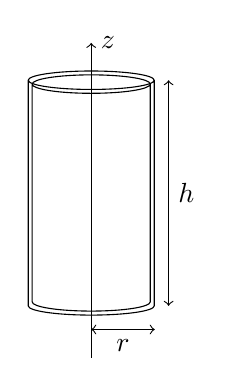
\begin{tikzpicture}
  \draw [->] (0,-2) -- (0,2) coordinate (a) node[right] {$z$};
  \node (a) [cylinder, shape border rotate=90, draw, minimum height=30mm, minimum width=15mm] {};
  \node (a) [cylinder, shape border rotate=90, draw, minimum height=31mm, minimum width=16mm] {};
  \draw [<->] ([xshift=5pt]a.before bottom) -- ([xshift=5pt]a.after top) node [midway, right] {$h$};
  \draw [<->] ([yshift=-5pt]a.bottom) -- ([yshift=-5pt]a.bottom -| a.before bottom) node [midway, below] {$r$};
\end{tikzpicture}
\end{center}

\begin{enumerate}

\item By considering one needle like mass at the origin one can integrate Gauss's law for Gravity inside a cylinder of height $h$ and radius $r$ as follows:
\[
	\oint  \grad \Phi \cdot \dd \va{S}= \int \div \grad \Phi (\va{x}) \dd[3]x = 4\pi \frac{G_N}{c^2} \int \rho(\va{x}) \dd[3]{x} = 4\pi \frac{G_N}{c^2} \dd{\mu} h
\]
Because of the symmetry of the problem one can say that $\grad\Phi$ will only be in the radial direction ad so only the side of the cylinder. So:
\[
	\grad \Phi = 2 \frac{G_N}{c^2} \frac{\dd{\mu}\va{r}}{r^2}
\]

\item By considering the cylindrical shell as made up of needles one can "simplify" the above integral as an integral over the plane of "needle-like" gravitational charges. This means that for a generic cylindrically symmetric stress tensor one can rewrite with the help of Fubini Theorem that:
\[
	\grad \Phi_{\mu\nu} (\va{x}) = 2 \kappa \int \dd[3]{y} T_{\mu\nu} \frac{(\va{x} - \va{y})}{\abs{\va{x} - \va{y}}^2}
\]
The best way to do formally do this is finding the actual Green's function for the needle like source. The equation for this case is:
\[
	\div G = \delta(x)\delta(y) \implies G = \frac{1}{2\pi} \frac{\va{r}}{r^2}
\]
and then by convolution with the new source term this becomes:
\[
	\grad \Phi_{\mu\nu} = 2\kappa \int \dd[2]{y'} T_{\mu\nu} (\va{x}) \frac{(\va{x} - \va{y})}{\abs{\va{x} - \va{y}}^2}
\]
which is the above stated result.

\item The stress tensor for a cylindrical shell rotating with angular velocity $\Omega$ is:
\[
	[T_{\mu\nu}(\va{x})] = \rho_0 \frac{\delta(r - R)}{r} c^2 \frac{\Omega R}{c} \begin{bmatrix}
		\frac{c}{\Omega R} &- \sin\phi & \cos\phi& 0 \\
		- \sin\phi & 0 & 0 & 0 \\
		 \cos\phi & 0 & 0 & 0 \\
		0 & 0 & 0 & 0 \\
	\end{bmatrix}
\]
Then to calculate the two terms required one has to evaluate:
\[
	\partial_y \Phi_{0x} (\va{0}) = 2 \kappa \rho_0 c\Omega R \int_0^{\infty}\int_0^{2\pi} \dd{r} \dd{\phi} \frac{\delta(r-R)}{r} \: \sin^2\phi = \kappa \mu c \Omega
\]
\[
	\partial_x \Phi_{0y} = -\kappa \mu \Omega c
\]

\begin{figure}[htbp]
   \centering
   \includegraphics[scale=0.65]{ypsilon.png} % requires the graphicx package
   \caption{Displacement in the $y$ direction. The simulation has been carried out with the following paramethers: $R=1\si{\meter}$, $v=\SI{1e5}{\meter\per\second}$, $\mu = \SI{1e20}{\kilo\gram\per\meter\cubed}$, $x_0 = 11\si{\meter}$ and $\dot{x}_0 = \SI{-1e5}{\meter\per\second}$.}
   \label{fig:ypsilon}
\end{figure}

\item
\begin{enumerate}[label=(\alph*)]
	\item Provided that all the other terms are zero one can find form $\Phi_{\mu\nu} = -\overline{h}_{\mu\nu} /4$ the perturbation to the metric. The function $\Phi_{\mu\nu}$ becomes:
	\begin{align*}
		\Phi_{0x} &=  \kappa \mu c \Omega y + \text{const.} \\
		\Phi_{0y} &= -\kappa \mu c \Omega x + \text{const.}
	\end{align*}
	which implies that, setting the constant to 0:
	\[
		\qty[\overline{h}_{\mu\nu}] = - 4\kappa \mu c \Omega \begin{bmatrix}
			0 & y & -x & 0 \\
			y & 0 & 0 & 0 \\
			-x & 0 & 0 & 0 \\
			0 & 0 & 0 & 0 \\
		\end{bmatrix} = \qty[h_{\mu\nu}]
	\]
	since it is a traceless matrix.
	
	\item The equations of motion become:
	\[
		\begin{cases}
			\ddot{t} = 0 \\
			\ddot{x} = 16 \kappa \rho_0 c \Omega\dot{y} \\
			\ddot{y} = - 12 \kappa \rho_0 c \Omega \dot{x} \\
			\ddot{z} = 0
		\end{cases}
	\]
	and considering for initial conditions a particle thrown from $(x_0>R, 0, 0)$ with a velocity $(\dot{x}_0, 0,0)$ one obtains for the solution a circular orbit centred in $(x_0, -\dot{x}_0/(8\kappa \rho_0 c \Omega) ,0)$ with a radius of $\dot{x}_0/(8\kappa \rho_0 c \Omega)$.
	A numerical simulation has been reported in Figure \ref{fig:ypsilon}.
	
	\item If one make a coordinate transformation to pass into some set of coordinates where the rotating cylinder is just a stationary cylinder then the distant objects observed starts rotating. This means that one can find a measurable quantity which differs in the two coordinates systems (the displacement of the far away stars). This is know as \textit{Mach's Principle} or \textit{Mach's Conjecture}.

\end{enumerate}

\end{enumerate}

\end{document}